\section{Problem Statement}%
\label{sec:problem}
The German parliament, called the \emph{Bundestag}, publishes the proceedings of
their meetings, as an effort to open up the political process to the common
people. These proceedings have been continously published since the inception of
the German Empire in 1871, when the parliament was called the \emph{Reichstag},
up to 1942; publishing resumed after the conclusion of World War 2 with the
inception of the Bundestag in 1949. Of course, the further back in the time you
go,the more difficult the documents become to use. While the more recent
documents are fully digital, documents prior to 1998 are scans of physical
documents and require optical character recognition, which becomes even more
problematic in the documents from the 1800s where a thick Gothic font is used.
\Cref{fig:pdf_page} shows a sample page from one of these proceedings; the
left column contains a continuation of a speech from the previous page as well
as two moderately sized speeches, while the right column contains a large number
of very short speeches. \Cref{fig:pdf_roi} shows the same page seen in
\cref{fig:pdf_page}, but with a number of regions of interest (manually)
colored in. Unfortunately this data is only available in a PDF format, which in
terms of internal representation is entirely unstructured. That means that none
of the rich structure highlighted in \cref{fig:pdf_roi} is actually
present in a computer-usable way.

\begin{figure}[p]
  \centering
  \includegraphics[page=16,height=0.95\textheight]{../pdfs/18001.pdf}
  \caption{A sample page from one of the Bundestag
    proceedings.\label{fig:pdf_page}}
\end{figure}
\begin{figure}[p]
  \centering
  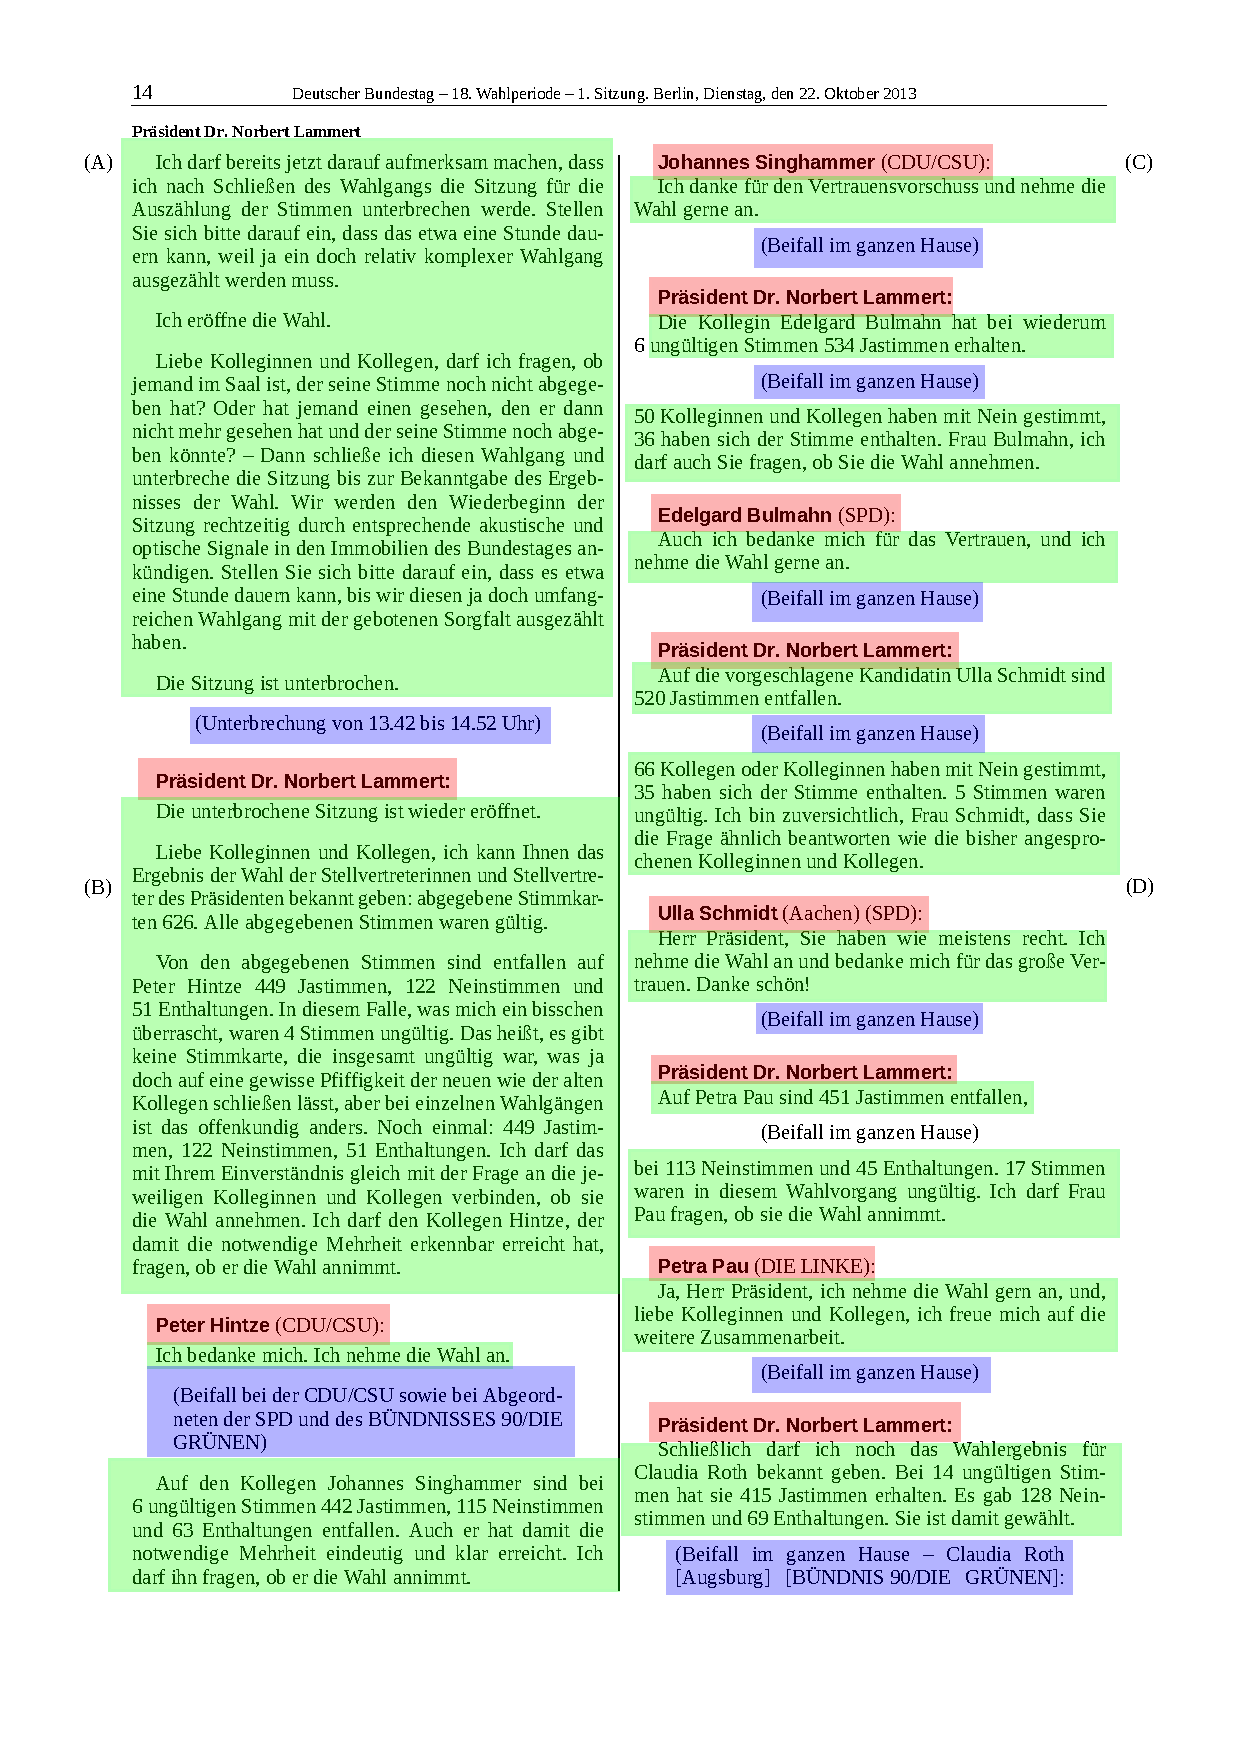
\includegraphics[height=0.85\textheight]{figures/pdf_roi.pdf}
  \caption{The same page as in Figure~\ref{fig:pdf_page}, hand-annotated with
    interesting regions that play a significant role in understanding the
    layout. The red regions are the headers the signify that someone is starting
    a speech, and contain information about who the speaker is. The blue
    regions are little interruptions (\emph{Heiterkeits}), often signifying
    approval or displeasure (the regularly seen \emph{Beifall} means applause).
  The green regions indicate plain blocks of text.\label{fig:pdf_roi}}
\end{figure}

The central problem in this thesis is the extraction of speeches from the
documents, transforming each document into a structured series of speeches that
can be serve as a useful entry point into further research. As a first step, the
structural layout (as in \cref{fig:pdf_roi}) will be extracted using
unsupervised clustering algorithms. The textual contents of the document are
then fed into supervised text classifier, where each piece of text is augmented
with the corresponding layout information previously obtained. More details on
this process will be supplied in \cref{sec:method}.

As annotating data by hand is an expensive process, a big focus is on limiting
the amount of required training data as much as possible; it would be preferable
if the system was able to learn sufficiently from a handful (say, less than 5)
of hand-annotated files.

\subsection{Dataset}
The dataset contains 11 hand-annotated documents, comprising 2052 positive
samples and 76,944 negative samples. The average document contains about 200
positive samples. Seeing as the source documents are PDF files, some
transformations are needed to extract text from them in a way that is suitable
for use as a machine learning dataset. This is not as trivial as it might seem,
given that PDF files only contain instructions for drawing certain characters at
certain coordinates, with no internal concept of paragraphs, lines or even
words.

For the supervised portion of the system, the PDF files are transformed using
the \texttt{pdftohtml} utility from the Poppler PDF rendering
library\footnote{https://poppler.freedesktop.org/}. This utility takes a PDF
file and uses a number of heuristics to output lines of text occurring
inside the file. In this context, a \emph{line} refers to any number of
characters that occur on the same height on a page while preserving reading
order (which is relevant when dealing with documents that have a two-column
layout) and is explicitly not the same as a sentence. These lines are output in
an XML format which includes metadata on the geometry of the line (position and
size) and its font. An example of a portion of text from the dataset and the
corresponding XML output from \texttt{pdftohtml} is shown in \cref{fig:example}.
Since this process is based on heuristics, it can and does go wrong; there are
instances of mistakes such as a single line being broken up into multiple XML
nodes, or lines of two side-by-side columns being taken as a single XML node.
This is not terribly common (the frequency of such errors is perhaps one per
file on average), but it does make the dataset inherently noisy and is one of
the issues that rule-based systems have trouble with.

For the unsupervised clustering, the PDF files are taken directly as input and
clustering is done using individual characters as the basic unit. This is just
as easy as clustering on the lines produced by \texttt{pdftohtml}, but has the
benefit of not being dependent on the imperfect line-extraction heuristics.

\begin{figure}[p]
  \centering
  \begin{subfigure}[b]{0.6\textwidth} 
    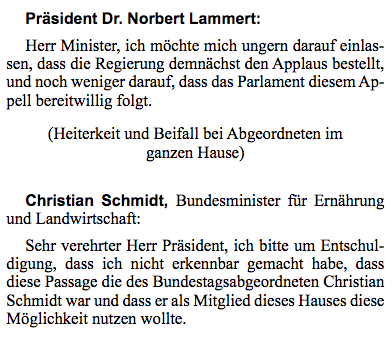
\includegraphics[width=\textwidth]{figures/source.png}
    \caption{A portion of the source PDF.\label{fig:source_pdf}}
    \vspace{1cm}
  \end{subfigure}
  \begin{subfigure}[b]{\textwidth}
    \begin{lstlisting}[language=xml, morekeywords={text}]
      <text top="122" left="125" width="143" height="16" font="3">
          Dr. Norbert Lammert 
      </text>
      <text top="122" left="269" width="83" height="17" font="4">
          (CDU/CSU):
      </text>
      <text top="142" left="125" width="328" height="17" font="4">
          Herr Alterspräsident, lieber Kollege Riesenhuber, ich
      </text>
      <text top="158" left="108" width="156" height="17" font="4">
          nehme die Wahl gerne an.
      </text>
      <text top="186" left="141" width="278" height="17" font="4">
          (Beifall im ganzen Hause – Abgeordnete aller
      </text>
      <text top="203" left="158" width="242" height="17" font="4">
          Fraktionen gratulieren dem Präsidenten)
      </text>
    \end{lstlisting}
    \caption{XML created by running \texttt{pdftohtml}, corresponding to the PDF
      excerpt in Figure~\ref{fig:source_pdf}. The contents of the \texttt{text}
      elements are used as inputs for the classification algorithm; the layout
      data contained in the properties is not used, as a separate software
    pipeline is used for the unsupervised clustering.\label{fig:source_xml}}
  \end{subfigure}
  \caption{A sample excerpt from a source PDF, along with its XML representation
    created by \texttt{pdftohtml}.\label{fig:example}}
\end{figure}

\FloatBarrier%
\subsection{Research Question}%
\label{sec:research_question}
A baseline model can be created by leaving out the clustering step, leaving us
with two models:
\begin{enumerate}
  \item A baseline model that classifies based on purely text
  \item A model that classifies based on both text and layout information
\end{enumerate}
There are two ways in which the second model can improve upon the baseline:
either it performs better (using a metric such as the F1 score), or it requires
less data to reach the same performance. This naturally leads to two research
questions:
\begin{researchquestion}
  Does augmenting a text classification system with layout information obtained
  by unsupervised clustering of the input data improve the F1 score of the
  classifier?
\end{researchquestion}
\begin{researchquestion}
  Does augmenting a text classification system with layout information obtained
  by unsupervised clustering of the input data allow the classifier to reach its
  peak performance using less input data?
\end{researchquestion}

%%% Local Variables:
%%% mode: latex
%%% TeX-master: "report"
%%% End:
